\documentclass[main.tex]{subfiles}
\begin{document}
\subsection{Find the simple roots, fundamental weights and the Dynkin diagram for the algebra in part (6.C)}
From part (6.C.b) we can obtain the simple roots by picking the two lowest roots. These are  $\alpha_1=(2,-2)$ and $\alpha_2=(0,2)$, then plotting the roots in terms of the simple roots
\begin{figure}[H]
\centering
\begin{tikzpicture}
\draw[->] (0,-3) -- (0,3) node[right] {$H_2$};
\draw[->] (-3,0) -- (3,0) node[right] {$H_1$};
\filldraw[black] (0,2) circle (2pt) node[right] {$\alpha_2$};
\filldraw[black] (2,2) circle (2pt) node[right] {$\alpha_1+2\alpha_2$};
\filldraw[black] (2,0) circle (2pt) node[below right] {$\alpha_1+\alpha_2$};
\filldraw[black] (2,-2) circle (2pt) node[right] {$\alpha_1$};
\filldraw[black] (0,-2) circle (2pt) node[right] {-$\alpha_2$};
\filldraw[black] (-2,-2) circle (2pt) node[left] {$-\alpha_1-2\alpha_2$};
\filldraw[black] (-2,0) circle (2pt) node[below left] {$-\alpha_1-\alpha_2$};
\filldraw[black] (-2,2) circle (2pt) node[left] {$-\alpha_1$};
\filldraw[black] (-0.1,0) circle (2pt) node[above left] {(0,0)};
\filldraw[black] (0.1,0) circle (2pt) node[above right] {(0,0)};
\draw[->, red] (2,0.07) -- (2,1.93);
\draw[->,red] (0,0.07) -- (0,1.93);
\draw[->,red] (2,-1.93) -- (2,-0.07);
\end{tikzpicture}
\end{figure}

The fundamental roots are given by 
\begin{equation}\label{eq:8fundamentalweights}
\frac{2\alpha^j.\mu^i}{{\alpha^j}^2}=\delta^{ij}.
\end{equation}
Letting $\mu^i=(a^i,b^i)$
\begin{align}
\mu^i.\alpha^1&=2a^i-2b^i\\
\mu^i.\alpha^2&=2b^i\\
{\alpha^1}^2&=8\\
{\alpha^2}^2&=4.
\end{align}
So 
\begin{align}
\frac{2\alpha^1.\mu^1}{8}&=\frac{1}{2}(a^1-b^1)=1\\
\frac{2\alpha^1.\mu^2}{8}&=\frac{1}{2}(a^2-b^2)=0\\
\frac{2\alpha^2.\mu^1}{4}&=b^1=0\\
\frac{2\alpha^2.\mu^2}{4}&=b^2=1.
\end{align}
Therefore, $\mu^1=(2,0)$, $\mu^2=(1,1)$.

For the Dynkin diagram
\begin{align}
\cos{(\theta_{\alpha^1,\alpha^2})}&=-\frac{\sqrt{p_1p_2}}{2}\\
&=\sqrt{\frac{(\alpha^1.\alpha^2)^2}{{\alpha^2}^2{\alpha^1}^2}}\\
&=-\frac{1}{\sqrt{2}}.
\end{align}
Then $\theta_{\alpha^1,\alpha^2}=\frac{3\pi}{4}$. So the Dynkin diagram is
\begin{figure}[H] 
\centering
  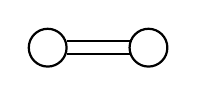
\begin{tikzpicture}[scale=.8]
   \draw[thick] (0,0) circle (.3);
     \draw[thick] (0.3, .1 ) -- +(1 ,0);
    \draw[thick] (0.3, -.1 ) -- +(1 ,0);
       \draw[thick] (1.6,0) circle (.3);
  \end{tikzpicture}
\end{figure}
Which is $C_2$ or $B_2$, $\mathfrak{so}(5)\cong\mathfrak{sp}(4)$.

\subsection{Show the algebra generated by $\sigma_a\otimes\mathbb{I}$ and $\sigma_a\otimes\eta_1$ is semisimple. Draw it's Dynkin diagram.}\label{Sec:8B}
We know that the simple roots of a simple Lie algebra are simply connected with atleast one other simple root in the root system and they obey $\alpha^i.\alpha^j<0$. One way of showing that the algebra is not simple, but semi-simple is to find the simple roots and then show that $\alpha^i.\alpha^j\nless0$. First we write out the commutation relations
\begin{align}
[\sigma_a\otimes\mathbb{I},\sigma_b\otimes\mathbb{I}]&=2\img\epsilon_{abc}\sigma_c\otimes\mathbb{I}\\
[\sigma_a\otimes\eta_1,\sigma_b\otimes\eta_1]&=2\img\epsilon_{abc}\sigma_c\otimes\mathbb{I}\\
[\sigma_a\otimes\mathbb{I},\sigma_b\otimes\eta_1]&=2\img\epsilon_{abc}\sigma_c\otimes\eta_1.
\end{align}
Therefore we pick the Cartan subalgebra as
\begin{equation}
\sigma_3\otimes\mathbb{I}=\begin{pmatrix}1&0&0&0\\0&1&0&0\\0&0&-1&0\\0&0&0&-1\end{pmatrix},\quad\sigma_3\otimes\eta_1=\begin{pmatrix}0&1&0&0\\1&0&0&0\\0&0&0&-1\\0&0&-1&0\end{pmatrix}.
\end{equation}
Which have eigenvalues $\lambda=\pm1$ and weights eigenvectors are
\begin{align}
x_1&=\begin{pmatrix}1\\1\\0\\0\end{pmatrix} \quad \mu_1=(1,1),\quad\\ 
x_2&=\begin{pmatrix}0\\0\\1\\1\end{pmatrix} \quad \mu_2=(-1,-1),\quad\\
x_3&=\begin{pmatrix}1\\-1\\0\\0\end{pmatrix} \quad \mu_3=(1,-1),\quad\\
x_4&=\begin{pmatrix}0\\0\\1\\-1\end{pmatrix} \quad \mu_4=(-1,1).
\end{align}
From which we may construct the simple roots $\alpha=(1,1)$, $\beta=(1,-1)$ and then $\alpha.\beta=0\nless0$ contrary to that of a simply connected Lie algebra. Thus the algebra is semi simple.
\begin{equation}
\cos{(\theta_{\alpha,\beta})}=\sqrt{\frac{(\alpha.\beta)^2}{(\alpha)^2(\beta)^2}}=0.
\end{equation}

So $\theta_{\alpha,\beta}=\frac{\pi}{2}$. So the Dynkin diagram is
\begin{figure}[H] 
\centering
  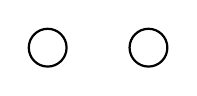
\begin{tikzpicture}[scale=.8]
   \draw[thick] (0,0) circle (.3);
       \draw[thick] (1.6,0) circle (.3);
  \end{tikzpicture}
\end{figure}
This algebra describes $A_1\times A_1$ or $\mathfrak{su}(2)\times\mathfrak{su}(2)$.

\subsection{Find the Cartan matrix and find the Dynkin coefficients}
We are given the Dynkin diagram 
\begin{figure}[H] 
\centering
  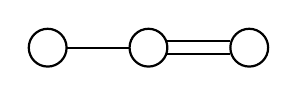
\begin{tikzpicture}[scale=.8]
   \draw[thick] (0,0) circle (.3);
     \draw[thick] (0.3, .1 ) -- +(1 ,0);
    \draw[thick] (0.3, -.1 ) -- +(1 ,0);
       \draw[thick] (1.6,0) circle (.3);
          \draw[thick] (-1.6,0) circle (.3);
              \draw[thick] (-0.3, 0 ) -- +(-1 ,0);
  \end{tikzpicture}
\end{figure}
with ${\alpha^1}^2={\alpha^2}^2$, ${\alpha^3}^2=1$.
\begin{align}
\cos{(\theta_{\alpha_1\alpha_2})}&=-\frac{1}{2}=-\sqrt{\frac{(\alpha_1.\alpha_2)^2}{(\alpha_1)^2(\alpha_2)^2}}\\
\cos{(\theta_{\alpha_2\alpha_3})}&=-\frac{1}{\sqrt{2}}=-\sqrt{\frac{(\alpha_2.\alpha_3)^2}{(\alpha_2)^2(\alpha_3)^2}}.
\end{align}
So $\alpha_1.\alpha_2=\alpha_2.\alpha_3=1$. The Cartan matrix is
\begin{equation}
A_{ji}=\frac{2\alpha^j.\alpha^i}{{\alpha^i}^2}=\begin{pmatrix}2&-1&0\\-1&2&-2\\0&-1&2\end{pmatrix}
\end{equation}
Which gives the Dynkin tree diagram
\begin{figure}[H]
\centering
\begin{tikzpicture}
  \node (max) at (2,10) {$(0,1,0)$};
  \node (a) at (2,8) {$(1,-1,2)$};
  \node (b) at (2,6) {$(-1,0,2)$};
  \node (c) at (0,6) {$(1,0,0)$};
  \node (d) at (-2,4) {$(1,0,1)$};
  \node (e) at (2,4) {$(-1,1,0)$};
  \node (f) at (-2,2) {$(2,-1,0)$};
  \node (g) at (0,2) {$(1,2,-2)$};
  \node (h) at (2,2) {$(0,-1,2)$};
  \node (min) at (0,0) {$(0,0,0)$};
  \draw (min) -- (g);
  \draw (h) -- (e);
  \draw (f) -- (d);
  \draw (a) -- (max);
  \draw [transform canvas={xshift=1.5em}] (b) -- (e);
  \draw [transform canvas={xshift=1.5em}] (a) -- (c);
  \draw [transform canvas={xshift=-1.5em}] (a) -- (b);
  \draw [transform canvas={xshift=1.5em}]  (c) -- (d);
  \draw [transform canvas={xshift=-1.5em}] (min) -- (f);
  \draw [transform canvas={xshift=1.5em}] (min) -- (h);
  \draw [transform canvas={xshift=-1.5em}] (g) -- (d);
  \draw [transform canvas={xshift=1.5em}] (g) -- (e);
  \draw [transform canvas={xshift=-1.5em}] (c) -- (e);  
\end{tikzpicture}
\end{figure}
\end{document}